%&pdflatex

\documentclass[12pt]{article}

\usepackage[spanish, es-tabla]{babel}
\usepackage{enumerate}
\usepackage{lscape}
\usepackage{vmargin}
\usepackage{pdfpages}
\usepackage{fancyhdr}
\usepackage{graphicx}
\usepackage{float}
\usepackage{titlesec}
\usepackage[bottom]{footmisc}
\usepackage[hidelinks]{hyperref}
\usepackage{listings}
\usepackage{color}
\usepackage{colortbl}
\usepackage{xcolor}
\usepackage{amsmath}
\usepackage{array}
\usepackage{svg}
\usepackage{pgfgantt}
\usepackage[T1]{fontenc}
\usepackage[sfdefault]{AlegreyaSans} %% Option 'black' gives heavier bold face
%% The 'sfdefault' option to make the base font sans serif
\renewcommand*\oldstylenums[1]{{\AlegreyaSansOsF #1}}


%*******************************************************************************
\extrarowheight = -0.3ex
\renewcommand{\arraystretch}{2.25}
\setpapersize{A4}
\hypersetup{
    colorlinks=true,
    linkcolor=blue,
    urlcolor=purple,
    citecolor=black, 
    linktocpage=true,
}
\definecolor{gray95}{gray}{.95}
\definecolor{gray75}{gray}{.75}
\definecolor{barblue}{RGB}{153,204,254}
\definecolor{groupblue}{RGB}{51,102,254}
\definecolor{linkred}{RGB}{165,0,33}
\lstset{
    frame=Ltb,
    framerule=0pt,
     aboveskip=0.5cm,
     framextopmargin=3pt,
     framexbottommargin=3pt,
     framexleftmargin=0.4cm,
     framesep=0pt,
     rulesep=.4pt,
     backgroundcolor=\color{gray95},
     rulesepcolor=\color{cyan},
     %
     stringstyle=\ttfamily,
     showstringspaces = false,
     basicstyle=\small\ttfamily,
     commentstyle=\color{cyan},
     keywordstyle=\bfseries\color{purple},
     %
     numbers=left,
     numbersep=15pt,
     numberstyle=\small,
     numberfirstline = false,
     breaklines=true,
}

%minimizar fragmentado de listados
\lstnewenvironment{listing}[1][]
   {\lstset{#1}\pagebreak[0]}{\pagebreak[0]}


\lstdefinestyle{C}
   {
       language=C++,
   }

\lstdefinestyle{python}
    {
        language=Python,
    }

\setcounter{secnumdepth}{4}
%*******************************************************************************
%   Adding a new level of section --> subsubsubsection
%******************************************************************************
\titleclass{\subsubsubsection}{straight}[\subsection]

\newcounter{subsubsubsection}[subsubsection]
\renewcommand\thesubsubsubsection{\thesubsubsection.\arabic{subsubsubsection}}
\renewcommand\theparagraph{\thesubsubsubsection.\arabic{paragraph}} % optional; useful if paragraphs are to be numbered

\titleformat{\subsubsubsection}
  {\normalfont\normalsize\bfseries}{\thesubsubsubsection}{1em}{}
\titlespacing*{\subsubsubsection}
{0pt}{3.25ex plus 1ex minus .2ex}{1.5ex plus .2ex}

\makeatletter
\renewcommand\paragraph{\@startsection{paragraph}{5}{\z@}%
  {3.25ex \@plus1ex \@minus.2ex}%
  {-1em}%
  {\normalfont\normalsize\bfseries}}
\renewcommand\subparagraph{\@startsection{subparagraph}{6}{\parindent}%
  {3.25ex \@plus1ex \@minus .2ex}%
  {-1em}%
  {\normalfont\normalsize\bfseries}}
\def\toclevel@subsubsubsection{4}
\def\toclevel@paragraph{5}
\def\toclevel@paragraph{6}
\def\l@subsubsubsection{\@dottedtocline{4}{7em}{4em}}
\def\l@paragraph{\@dottedtocline{5}{10em}{5em}}
\def\l@subparagraph{\@dottedtocline{6}{14em}{6em}}
\makeatother

\setcounter{secnumdepth}{4}
\setcounter{tocdepth}{4}

%*****************************************************************************

\begin{document}

  \begin{titlepage}
    \centering
   {\bfseries\Large Universidad Carlos III de Madrid \par}
    \vspace{5cm}
    {\scshape\Huge Informe del Trabajo de Evaluación del Bloque 2 \par}
    \vspace{2cm}
    {\itshape\Large Diseño de circuitos electrónicos para comunicaciones}
    \vfill
    {\Large Autores: \par}
    \vspace{1cm}
    {\Large Markel Serrano y Daniel Theran}
    \vfill
    {\Large 20 de Noviembre del 2022 \par}
  \end{titlepage}

  %\tableofcontents
  %\newpage
  
  \section{Apartado 1}
    
    \paragraph*{}
    En el primer apartado se pide calcular la SNR a la entrada y la salida del LNA del circuito para dos valores de entrada dados, -30 y -70 dBm.
    Para ello, y como puede verse en los cálculos anexados, primero debe calcularse la SNR de entrada del LNA. Para ello, se divide la potencia
    de la señal de entrada entre la potencia del ruido térmico a la entrada, como puede verse en la fórmula, y se cambia de unidades lineales a logarítmicas.
    
    \paragraph*{}
    Una vez calculada la SNR de entrada para ambos casos, basta con restar la figura de ruido del LNA para obtener las señales SNR de salida correspondientes.


  \section{Apartado 2}
    
    \paragraph*{}
    En el segundo apartado se pide calcular la figura de ruido del mezclador y etapas siguientes para que la figura de ruido total del receptor no supere nunca 10dB.
    Como puede verse en el diagrama de bloques anexado, se ha modelado el circuito con una bifurcación en dos líneas (la línea I y la Q, como corresponde a un receptor en cuadratura).
    Ambas líneas son simétricas exceptuando un desfase de 90º, pero los bloques que las componen son los mismos. Más concretamente, cada línea se compone
    de un mezclador, un filtro paso bajo y un controlador automático de ganancia (AGC).
    
    \paragraph*{}
    Para resolver este apartado, se ha de tener en cuenta que la figura de ruido más importante, debido a la formula de Friis, es la del LNA, la cual es conocida (de 2,4 dB).
    Por tanto, pueden modelarse el resto de bloques como uno solo, y encontrar la figura de ruido máxima de este simplemente despejando de la formula de Friis. Así,
    se consigue una figura de ruido máxima posible para ese bloque equivalente de 25,18 dB.


  \section{Apartado 3}
  
    \paragraph*{}
    En el tercer apartado se pide calcular las ganancias mínima y máxima del AGC, suponiendo el caso de máxima ganancia para -70 dBm a la entrada.
    Sabiendo que el AGC mantiene una salida 1 Vrms, y que su margen de ganancias es de 40 dB, basta con calcular la ganancia máxima, que será de 130 dBm
    (la diferencia entre los 60 dbM a la salida correspondientes a 1 Vrms y la suposición de -70 dBm de la entrada.) Después, se aplica el rango de 40 dB que
    caracteriza al AGC y se obtiene la ganancia mínima, de 90 dB para este caso.
 

  \section{Apartado 4}
  
    \paragraph*{}
    El cuarto apartado se pide diseñar un AGC lineal en dB con un detector de valor rms, y calcular la tensión de referencia necesaria.
    Para ello, se diseña primero un diagrama de bloques lineal en el que se introduce un detector de envolvente, un bloque de paso a potencia,
    un mezclador para introducir la tensión de referencia y un integrador. Así, pasando este diagrama de bloques lineal a logarítmico, despejamos primero
    la ecuación que relaciona la entrada Vi con la salida Vo para despejar la Ley de Control y después se despeja la ecuación del mezclador que relaciona nuestro
    tono de prueba con Vo. De esta forma, y analizando dicho caso en régimen permanente, encontramos que la tensión de prueba necesaria para mantener la salida dada es de 3 dB (es decir, 
    1,41 Vrms).


  \section{Apartado 5}
    
    \paragraph*{}
    A partir del quinto apartado, se pide realizar diferentes simulaciones y pruebas en LTSpice para probar el funcionamiento del bloque correspondiente al mezclador pasivo y el 
    filtro paso baso, los cuales son iguales en las dos ramas del circuito receptor. El circuito a analizar es el siguiente: 

    \begin{figure}[H]
      \centering
      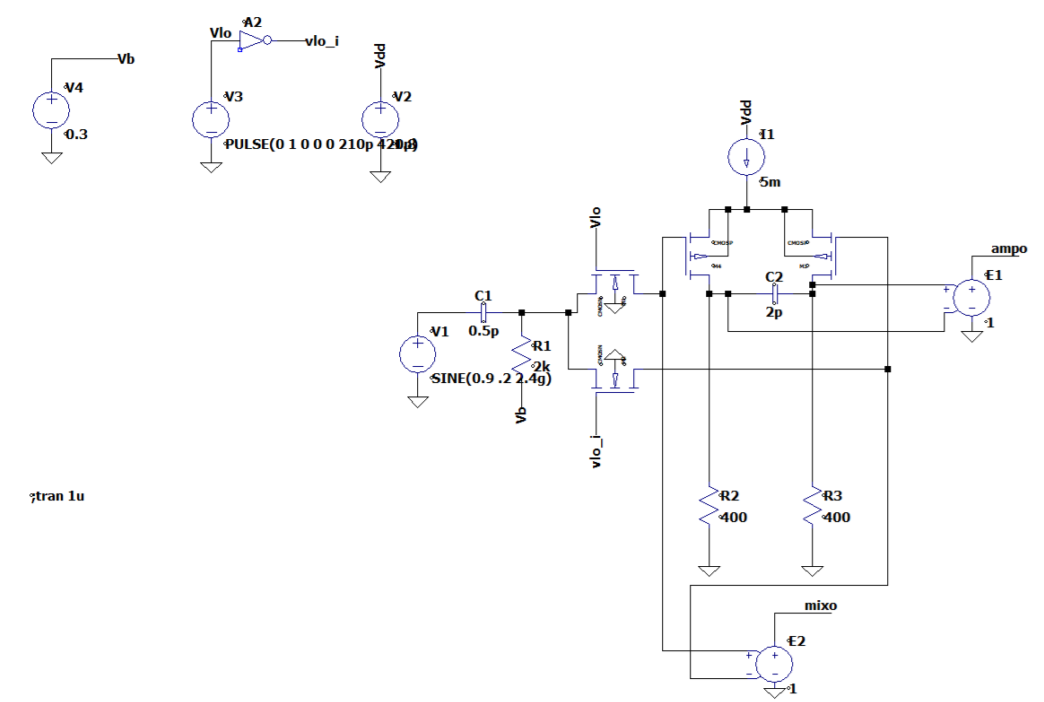
\includegraphics[width=1\linewidth]{img/circuitoRecep.png}
      \caption{Mezclador y filtro paso bajo en LTSpice.}%
      \label{fig:recep}
    \end{figure}
    
    \paragraph*{}
    El mezclador pasivo se simula con dos transistores CMOS que actúan como interruptores. Dado que queremos ver la señal resultante tanto del amplificador como de la etapa de 
    muestreo (salida ampo y mixo respectivamente), tenemos que elegir una frecuencia de muestreo de los interruptores que esté cerca de la frecuencia fundamental de la señal de 
    entrada pero que no sea la misma ya que veríamos a la salida una señal continua. Además, hay que satisfacer la banda de funcionamiento del LNA, por lo que el margen de 
    frecuencias de muestreo está entre los 2.38 GHz y los 2.42 GHz. 

    \paragraph*{}
    Simulando el circuito para las dos frecuencias anteriormente mencionadas, obtenemos las siguientes salidas: 

    \begin{figure}[H]
      \centering
      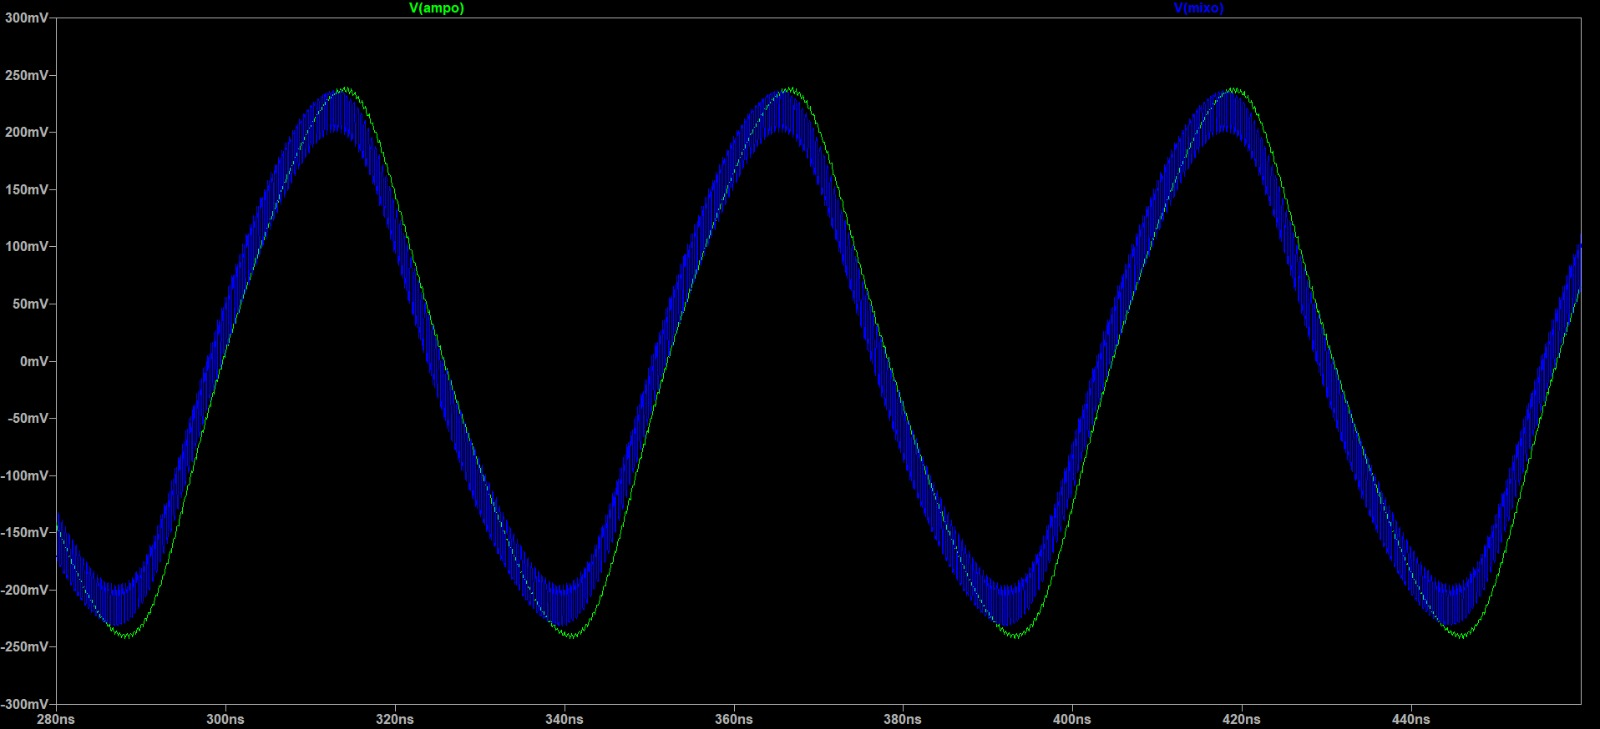
\includegraphics[width=1\linewidth]{img/salida238ghz.jpeg}
      \caption{Salida mixo y ampo para una frecuencia de muestreo de 2.38 Ghz}%
      \label{fig:238ghz}
    \end{figure}
    
    \begin{figure}[H]
      \centering
      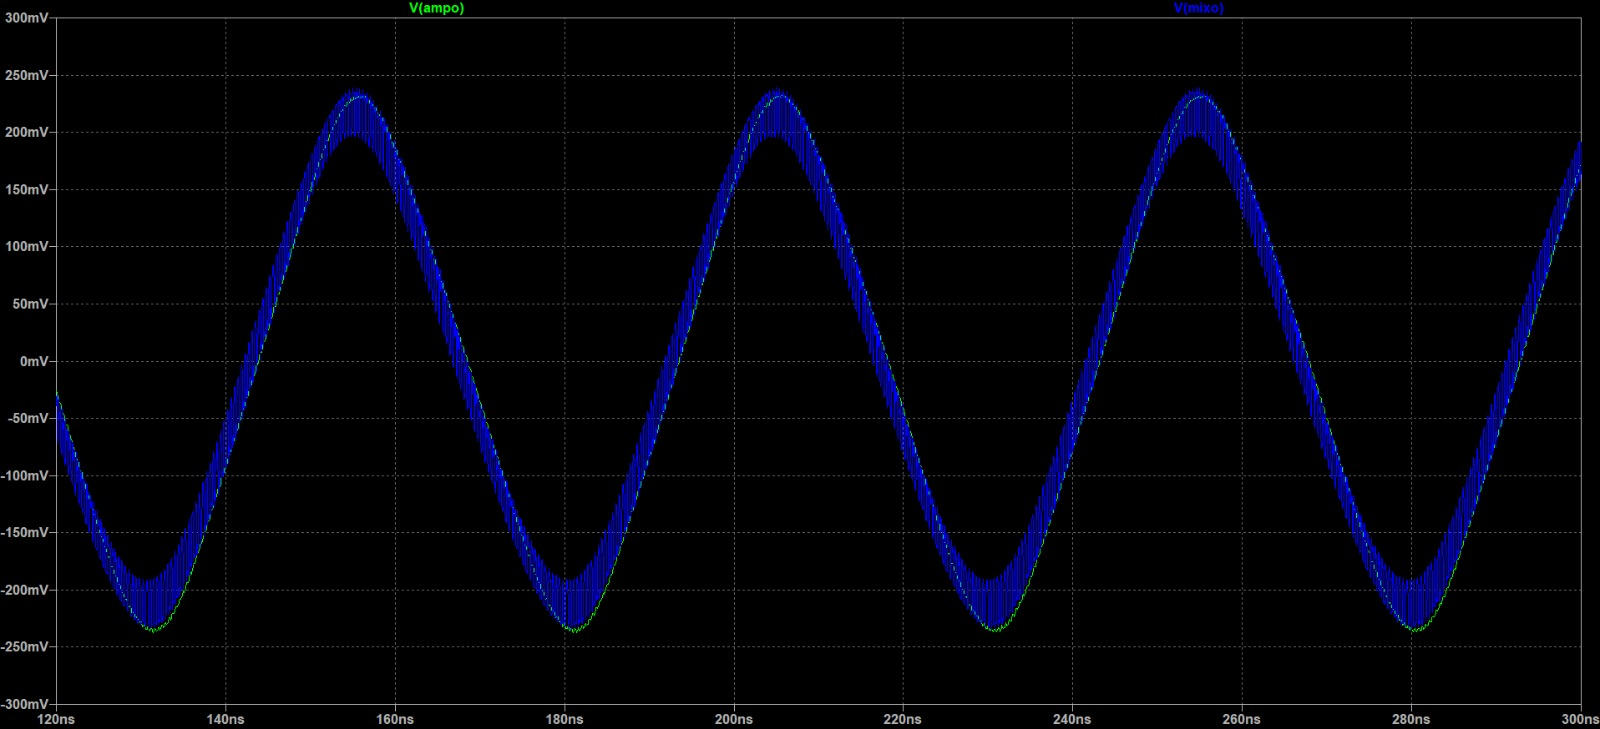
\includegraphics[width=1\linewidth]{img/salida242ghz.jpeg}
      \caption{Salida mixo y ampo para una frecuencia de muestreo de 2.38 Ghz}%
      \label{fig:242ghz}
    \end{figure}
    
    \paragraph*{}
    En las figuras anteriores podemos ver como la salida mixo (función de color azul) corresponde como a la diferencia de la señal de entrada muestreada. Cuando muestreamos a una
    frecuencia ligeramente inferior (2.38 GHz) a la frecuencia fundamental de la señal de entrada, nos encontramos con un pequeño desfase en la señal y por el contrario con una frecuencia un 
    poco mayor (2.42 GHz) el desfase es menor. 

    \paragraph*{}
    Cabe mencionar que en el análisis temporal de la señal de salida ampo, se puede observar la señal un tanto distorsionada y esto se debe a los ruidos que se le añaden a la misma. Sin embargo, 
    no podemos diferenciar qué ruidos exactamente están presentes ya que vemos una mezcla de varios posibles como el ruido de fase o el ruido térmico.  


  \section{Apartado 6}

    \paragraph*{}
    En este apartado vamos a realizar un análisis de ruido del circuito, por que necesitamos hacer un barrido AC para calcular el valor rms del ruido en las dos salidas del circuito.
    Para ello primero sustituimos interruptores por sus respectivas resistencias equivalentes en conducción. Una vez adaptado el circuito, pasamos a realizar una simulación de ruido 
    del mismo y obtenemos los siguientes resultados: 

    \begin{figure}[H]
      \centering
      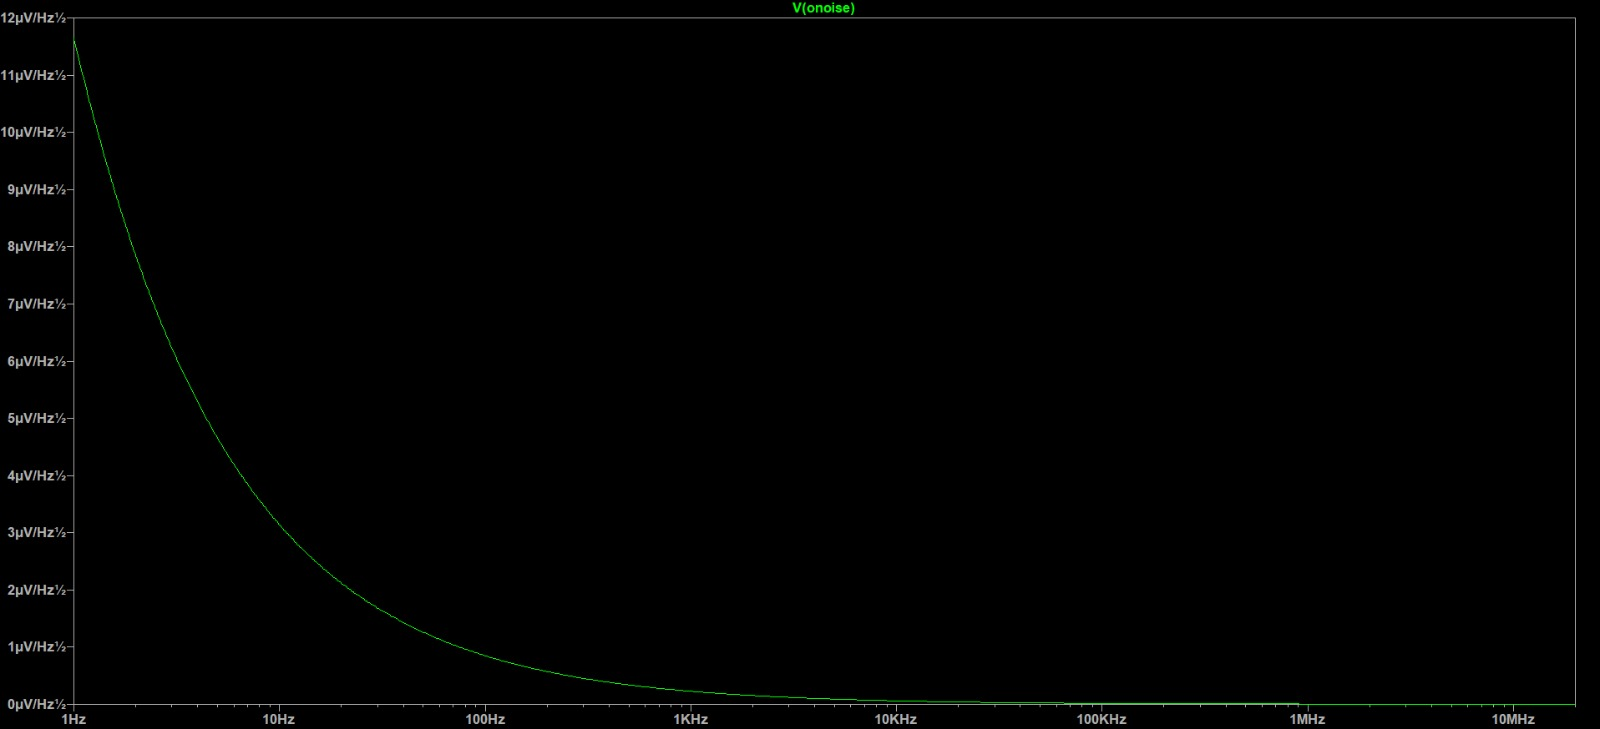
\includegraphics[width=1\linewidth]{img/ruidoampo.jpeg}
      \caption{Ruido en la salida ampo}%
      \label{fig:ruidampo}
    \end{figure}
    
    \begin{figure}[H]
      \centering
      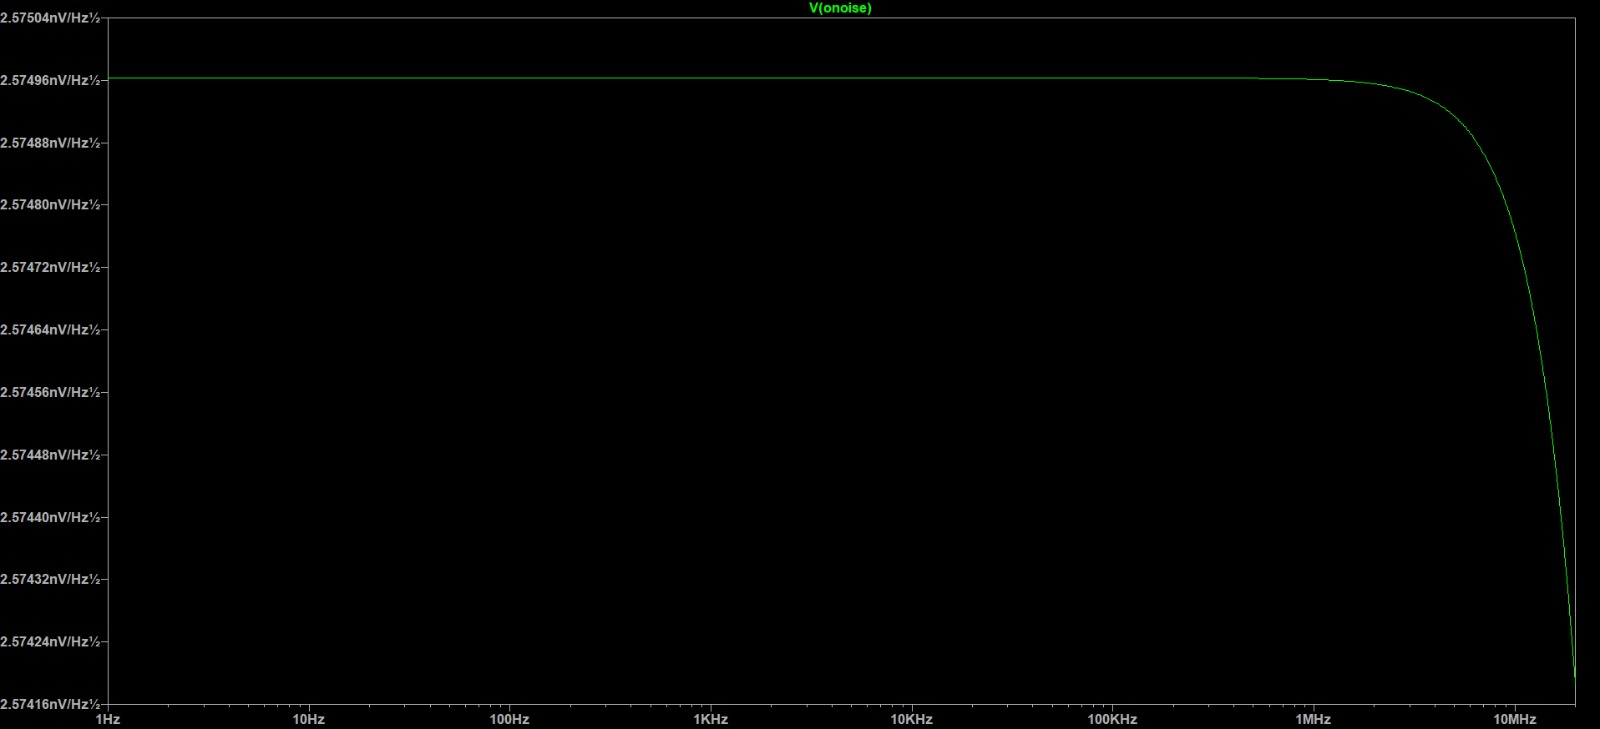
\includegraphics[width=1\linewidth]{img/ruidomixo.jpeg}
      \caption{Ruido en la salida mixo}%
      \label{fig:ruidmixo}
    \end{figure}
    
    \paragraph*{}
    Como vemos obtenemos dos salidas bastante diferentes y es debido a los ruidos que toman parte en cada etapa. En la salida mixo, lo que apreciamos es básicamente ruido térmico que 
    como vemos una vez superado el ancho de banda de operación se empieza a atenuar. Sólo vemos ruido térmico debido a que en ésta salida no toma parte ningún elemento capacitivo que 
    introduzca ruido flicker. 

    \paragraph*{}
    En la salida ampo, podemos apreciar tanto el ruido flicker que introducen los transistores CMOS , el cual es dominante hasta aproximadamente los 11 kHz. Después vemos ruido térmico el cual domina hasta el final y del 
    cual no apreciamos la etapa de atenuación del mismo por que es filtrado por el filtro paso bajo del sistema. 
    
    \paragraph*{}
    Lo último que se pide en este apartado es obtener el valor rms del ruido a la salida y ver si la figura de ruido resultante de este bloque cumple las condiciones que se calcularon 
    en el apartado 2. Para ello integramos la señal de ruido en la salida ampo entre 0 y 20 MHz, y obtenemos lo siguiente:

    \begin{figure}[H]
      \centering
      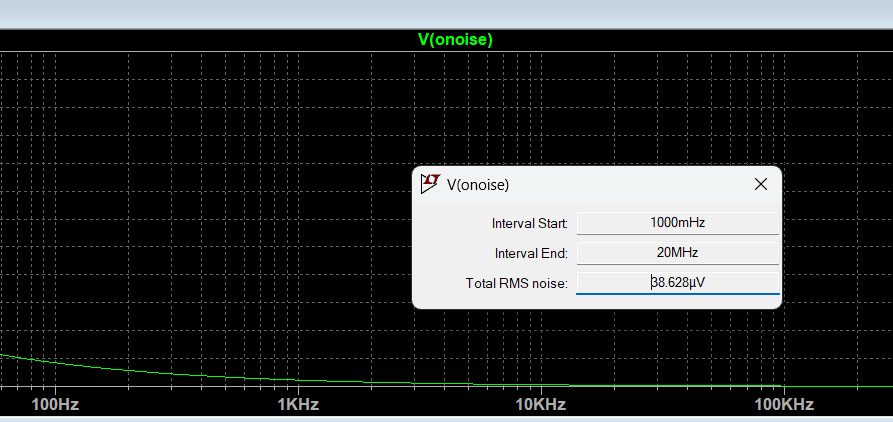
\includegraphics[width=1\linewidth]{img/rmsruido.png}
      \caption{Valor RMS del ruido en la salida ampo}%
      \label{fig:ruidorms}
    \end{figure}
    
    \paragraph*{}
    Con el valor obtenido realizamos los cálculos correspondientes para obtener la figura de ruido del bloque. Para ello calculamos la SNR a la entrada y a la salida del bloque mezclador + filtro, 
    y al restarlas obtendremos la figura de ruido teórica según las simulaciones. 
    
    \paragraph*{}
    Como podemos ver la figura de ruido obtenida es de 29.86 dB, valor que supera el límite que se impuso en el apartado 2 para obtener una figura de ruido total a la salida de 10 dB. Por lo que se 
    debería adaptar el circuito para reducir el ruido interno que genera este bloque. Los cálculos correspondientes a este apartado se encuentran en el anexo. 

  \section{Anexo: Desarrollo de los cálculos utilizados}
    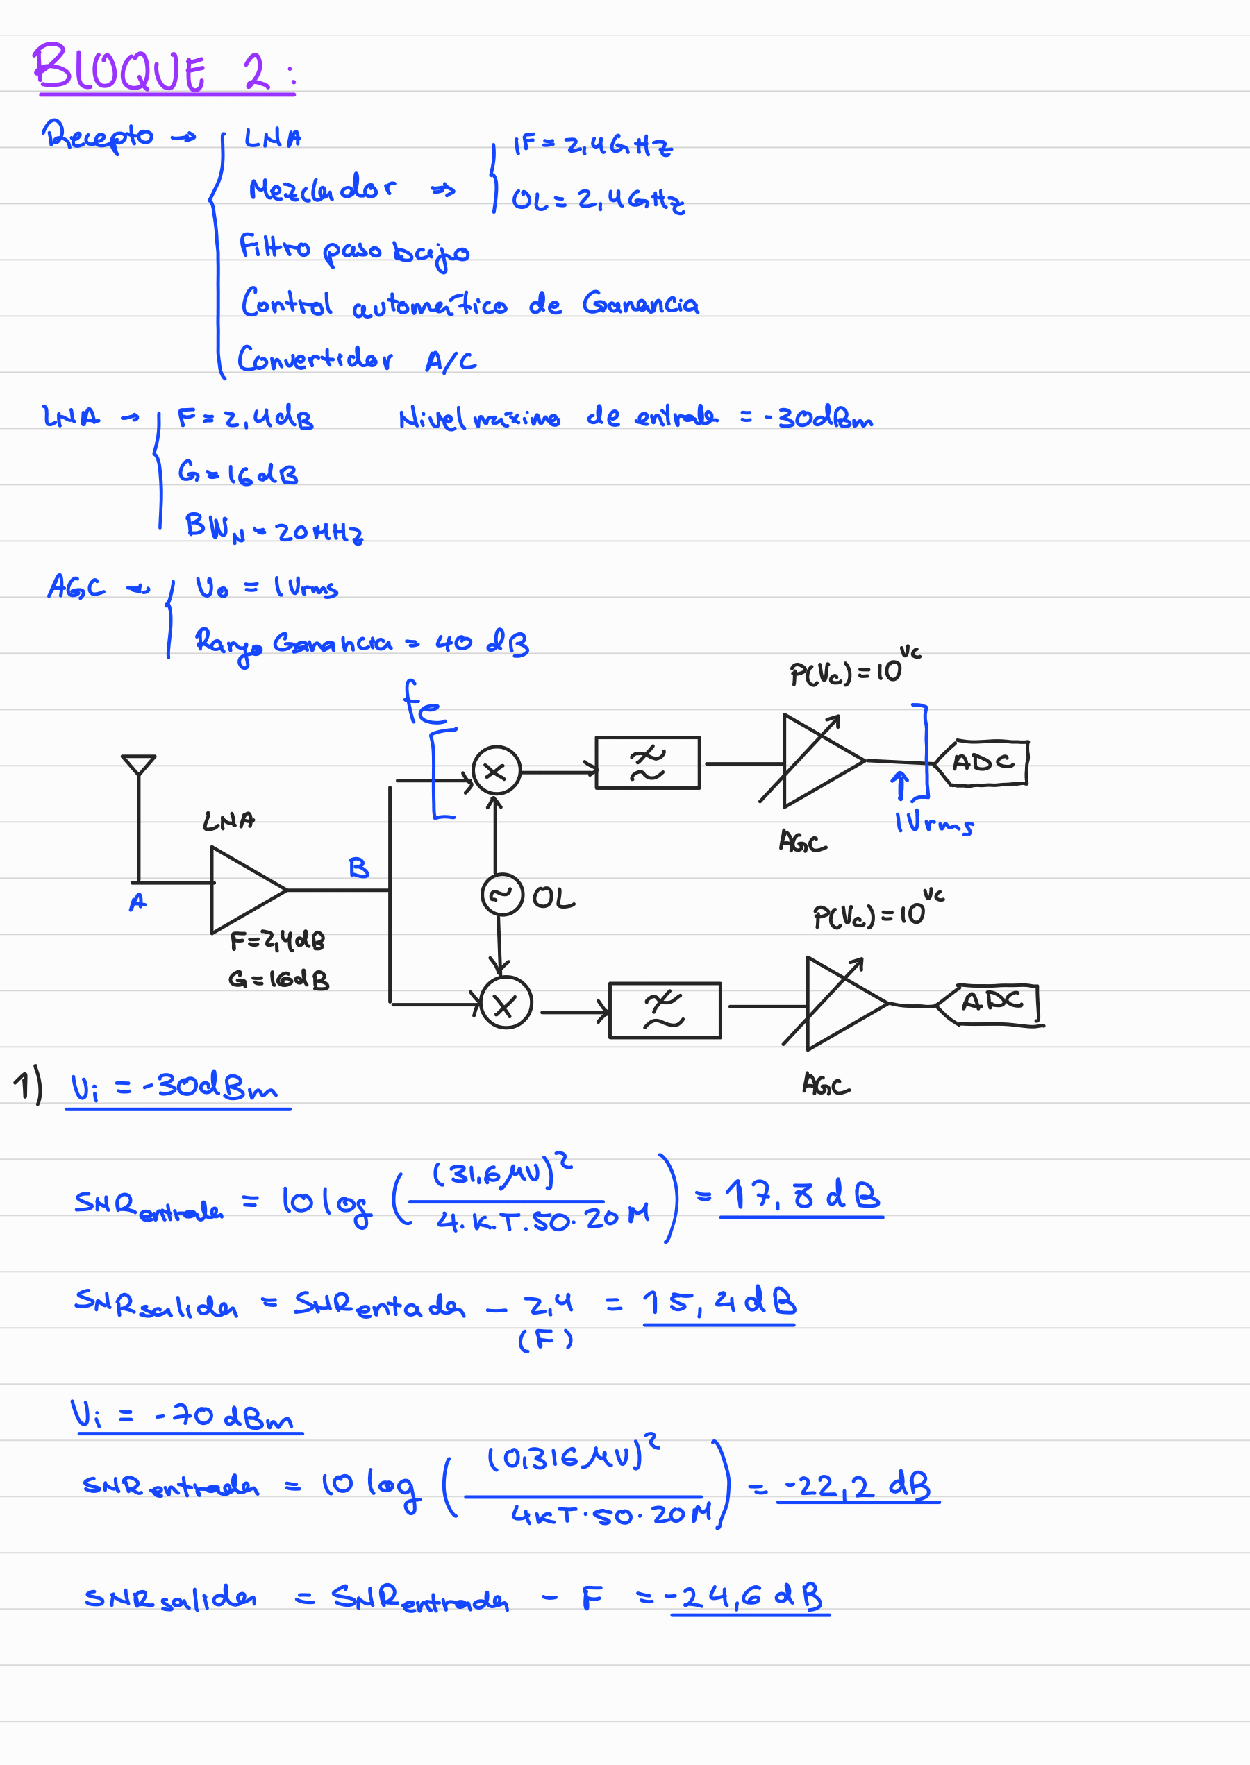
\includepdf[pages=-,pagecommand={},width=1.2\textwidth,offset= 2.5cm -2cm]{img/Ejercicio_Bloque_2.pdf}
  
 
\end{document}
